\documentclass{apuntes}

\usepackage{tikztools}
\usepackage{tikz-3dplot}
\usepackage{textcomp}
\usepackage{tikz-qtree}
\usepackage{changepage}
\usepackage{listings}
\usepackage{graphicx}
% subfiguras
\usetikzlibrary{arrows}

\newcommand{\theauthor}{}
\newcommand{\thetitle}{Memoria P2\\Criptografía}
\newcommand{\rightheader}{Memoria P2}
\newcommand{\leftheader}{UAM - 2015/2016}

% Si no compila y el directorio tikzgen está creado, quitar estas dos sentencias.
%\precompileImages
%\precompileTikz

\title{Criptografía}
\author{Cristina Kasner Tourné\\Jose Antonio García del Saz}
\date{Curso 2015 - 2015 C1}

% Paquetes adicionales

% --------------------

\newcommand{\cte}{\text{Cte}}

\begin{document}
\pagestyle{plain}
\maketitle
%\abstract{Porque los apuntes de Chamizo son demasiado fáciles}

\tableofcontents
\newpage
% Contenido.
\chapter{Ejercicios}
\section{Ejercicio 1-Seguridad perfecta}

En este ejercico nos piden implementar un programa que compruebe la seguridad perfecta.

Recordamos la definición de seguridad perfecta:

\begin{defn}[Seguridad Perfecta]
	Decimos que un criptosistema tiene seguridad perfecta si cumple:
	$$P_p(x|y) = P_p(x)$$
	Esto quiere decir que el conocimiento de texto cifrado no nos da ninguna información sobre el texto plano.
\end{defn}

Para esto hemos creado un fichero \textit{probabilidad.c} en el que implemetamos las funciones que calculan esas probabilidades.

La probabilidad $P_p(x)$ la calculamos recorriendo el fichero que tiene el texto plano y llevando la cuenta de las veces que aparece la letra i. 

\lstset{language=C, breaklines=true, basicstyle=\footnotesize}
\begin{lstlisting}


	while((l=fgetc(f))!=EOF){
		prob[l-65]++;
		longText++;
	}


\end{lstlisting}


Luego dividimos ese número entre la longitus del texto.

La probabilidad $P_p(x|y)$ la calculamos de la misma forma solo que contabilizando a la vez los caracteres del mensaje en plano y el mensaje cifrado.

\begin{lstlisting}


	while((c=fgetc(cifrado))!=EOF){
		p = fgetc(plano);
		prob[p-65][c-65]++;
		cantLetra[c-65]++;
	}
	
\end{lstlisting}

Y finalmente dividimos entre el número de veces que aparece en el texto cifrado la letra correspondiente.

En la práctica podemos probar la seguridad perfecta con dos casos distintos.

\begin{itemize}
	\item claves equiprobables
	\item claves no equiprobables
\end{itemize}

Para generar las claves equiprobables utilizamos la función random de C.

Para las claves no equiprobables hemos escrito el siguiente código:


\begin{lstlisting}


	for(i=0; i<2;i++){
		if((clave>m/2)==0){
			clave = rand() % m;
		}else break;
	}
	
	
\end{lstlisting}



De esta forma es mucho más probable que mi clave sea una clave menor que m/2 que mayor. 

Además obligamos a que la b también pertenezca a las unidades de m.

Los resultados obtenidos tras probar el código son:

\begin{center}
	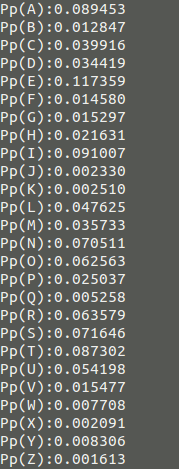
\includegraphics[width=90pt]{ProbabilidadesSimp.png}
\end{center}


\newpage
\textbf{Claves equiprobables}

\begin{center}
	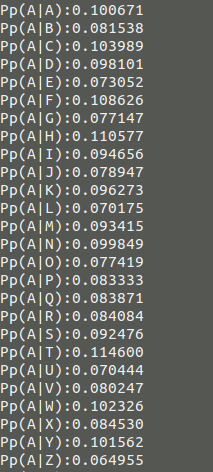
\includegraphics[width=100pt]{ProbA.png}
	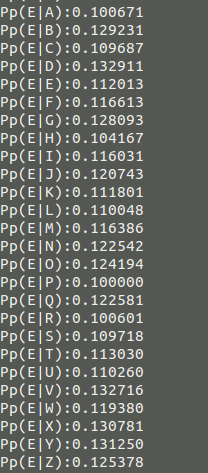
\includegraphics[width=98pt]{ProbE.png}
	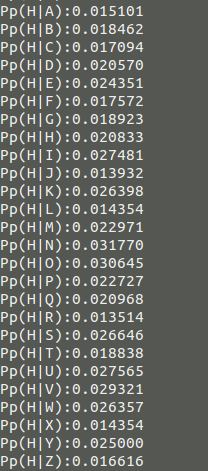
\includegraphics[width=98pt]{ProbH.png}
\end{center}

En estos ejemplos podemos ver que las probabilidades condicionadas son muy parecidas y todas tienen un valor muy cercano al de la probabilidad de la letra.

Una de las razones por las que el resultado no es exacto es que la función rand() de C no da resultados exactamente equiprobables.

\textbf{Claves no equiprobables}

\begin{center}
	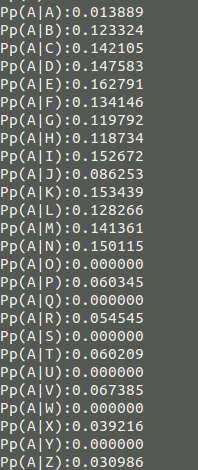
\includegraphics[width=102pt]{ProbANE.png}
	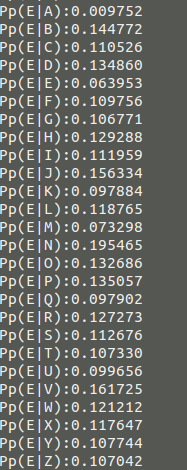
\includegraphics[width=96pt]{ProbENE.png}
	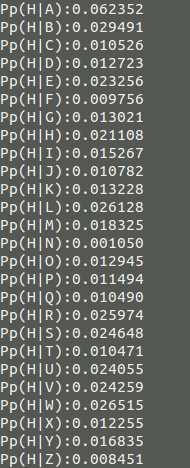
\includegraphics[width=98pt]{ProbHNE.png}
\end{center}

Vemos como estos resultados se distan mucho más que cuando utilizabamos claves probables.


\section{Ejercicio 2-Implementación del DES}

Para implementar el DES hemos creado un fichero que se llama \textit{funcionesDES.c} en el que están todas las funciones necesarias para el método.

Como sabemos el DES funciona a través de permutaciones y sustituciones(cajas-S), por esto no es ninguna sorpresa que el grueso de las funciones de \textit{funcionesDES.c} sean permutaciones y sustituciones.

Vamos a explicar ambas.

\begin{itemize}
	\item Permutaciones
	
	La idea de las funciones de permutación es la siguiente:
	
	Guardo el número que leo en la matriz de permutación, que es la posición del bit que va a ir en esa posición.
	
	Miro si ese bit es un 0 (positions[bit\%8] tiene un 1 en el bit que estoy mirando).
	
	Si es un 0 no hago nada ya que he inicializado permutation a 0.
	
	Si no es un cero meto en desired bit un 1 en la posicion apropiada y hago un 
	XOR con el byte que ya hubiera en permutation, de forma que solo cambio el bit deseado.
	
	Adjuntamos el código de una de las funciones de permutación para que se entienda mejor.
	
	\begin{lstlisting}
	
	int bit, newpos;
	unsigned char desiredbit;
	for (bit = 0; bit < 56; bit++) {
	
		newpos = ((int)PC1[bit])-1;
		desiredbit = input[newpos/8] & Positions[newpos%8]; 
		if (desiredbit != 0) {
			desiredbit = Positions[bit%8];
			permutation[bit/8] = desiredbit ^ permutation[bit/8];
		}
	}
	
	\end{lstlisting}
	
	\item Sustituciones $\rightarrow$ Cajas-S
	
	En esta función básicamente vamos rotando los bits para obtener la fila y la columna y obtenemos el resultado de las cajas-S de la siguiente forma:
	
	\begin{lstlisting}
	
	if((caja%2)==0){
		aux =S_BOXES[caja][posrow][poscolaux] <<4;
	}else{
		output[caja/2] = S_BOXES[caja][posrow][poscolaux];
		output[caja/2] =  output[caja/2] ^ aux;
		aux = 0;
	}
	
	\end{lstlisting}
	
	Esto es porque nuestra función devuelve una cadena de caracteres, cada caracter son 8 bits pero las cajas-S devuelven 4 bits por lo que vamos guardando los resultados de dos en dos.
	
\end{itemize}

Para encriptar se tiene que ejecutar el código tal y como indica el enunciado.

La clave para desencriptar aparece por terminar cuando encriptas.

Vamos a ver un ejemplo:

\begin{center}
		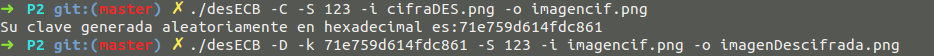
\includegraphics[width=400pt]{EjecutaDES.png}
\end{center}



\section{Ejercicio 3c y 4b -Estudiar la linealidad de las cajas-S del AES y del DES}
Las cajas de sustitución (cajas S) constituyen la piedra angular en criptografía para lograr que los
cifradores por bloque exhiban la ineludible propiedad de no linealidad.

 En efecto, si la o las cajas S
de un determinado cifrador por bloque no alcanzan una alta no linealidad, entonces se considera que
tal algoritmo no podrá ofrecer una seguridad adecuada para impedir que información confidencial
pueda ser develada por entidades no autorizadas.

Dada su definición, es claro que el número de funciones booleanas elegibles para diseñar una caja S de n bits de entrada y m bits de salida está dado por $2^{m\cdot 2^n}$ , de tal manera que aun para valores moderados de n y m el tamaño del espacio de búsqueda de este problema tiene un tamaño desmesurado.

Sin embargo, no todas las funciones booleanas son apropiadas para construir buenas cajas S.

Además de la ya mencionada propiedad de no linealidad,algunas de las principales propiedades criptográficas requeridas para dichas funciones booleanas incluyen: balance, alto grado algebraico, criterio de avalancha estricto, orden de inmunidad, etcétera.

Durante el desarrollo de esta práctica hemos aprovechado las cajas S de los algoritmos DES y AES para crear dos rutinas en C que demuestran la no linealidad de estas funciones booleanas. Estas dos rutinas han sido llamadas \textbf{linealidadSBoxesDES} y \textbf{linealidadSBoxesAES}

 Ambas rutinas reciben como argumento de ejecución "-n N", donde N es un número natural que indica el número de veces
que se quiere probar la no linealidad. La salida de estos dos programas se incluye a continuación para N=10:

\begin{figure}
	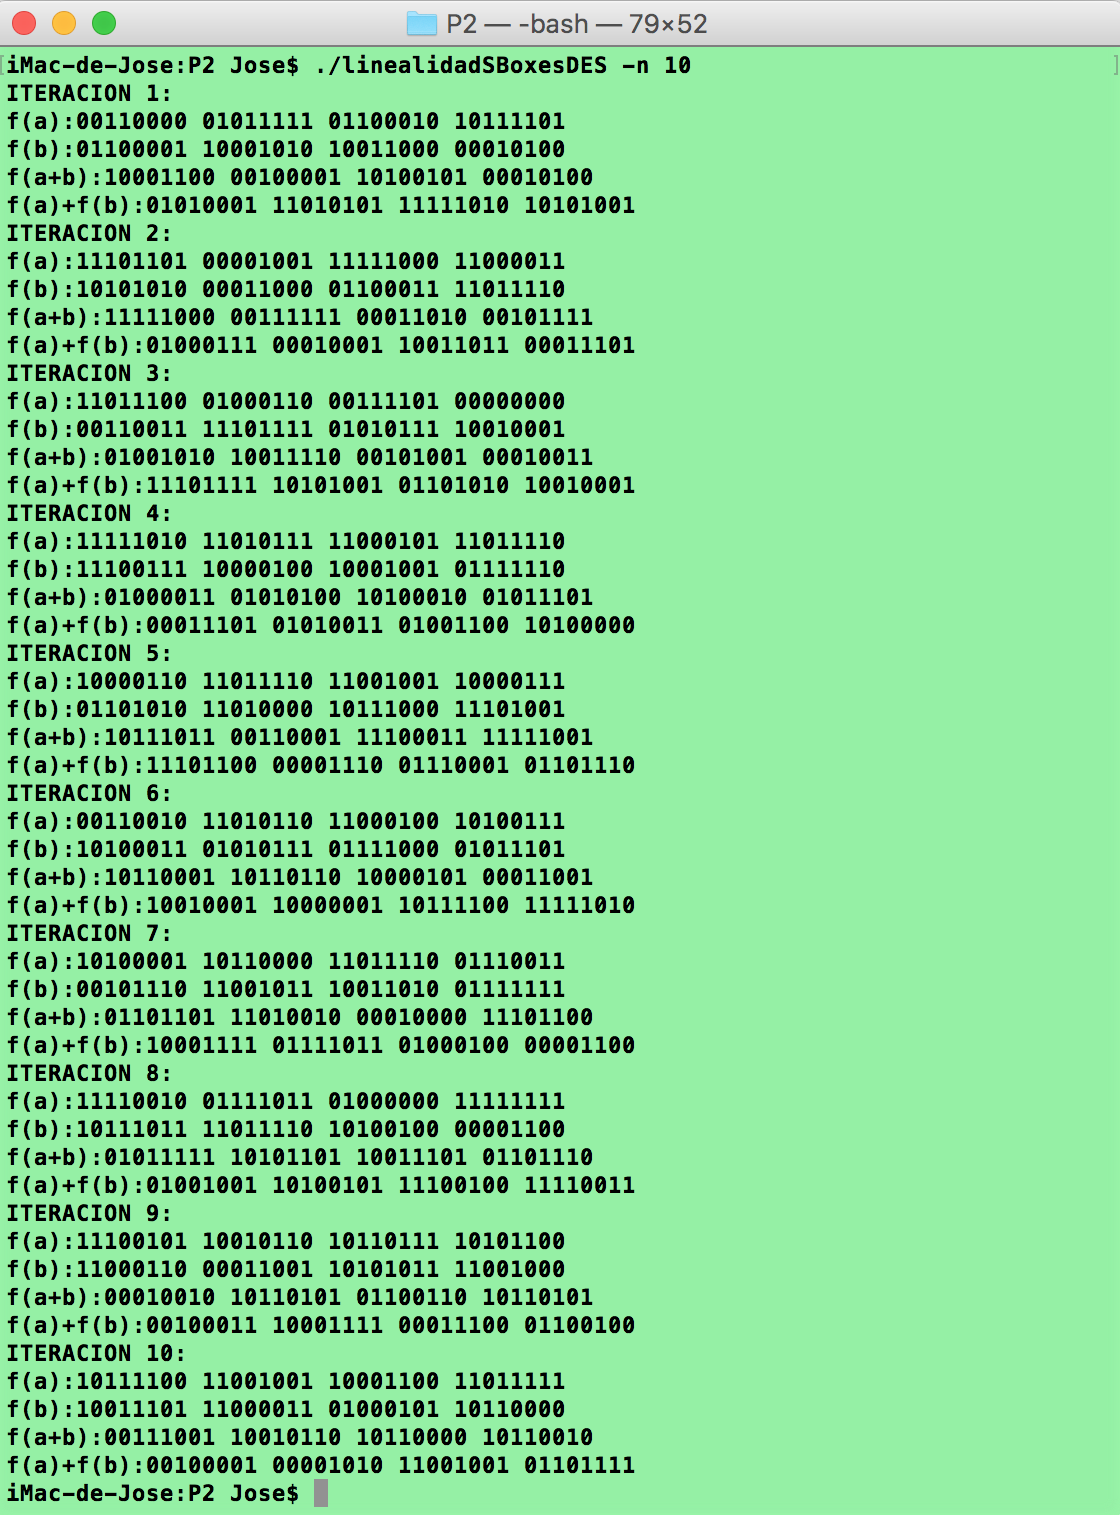
\includegraphics[width=200pt]{line2.png}
	\caption{No linealidad del DES}
\end{figure}

\begin{figure}
	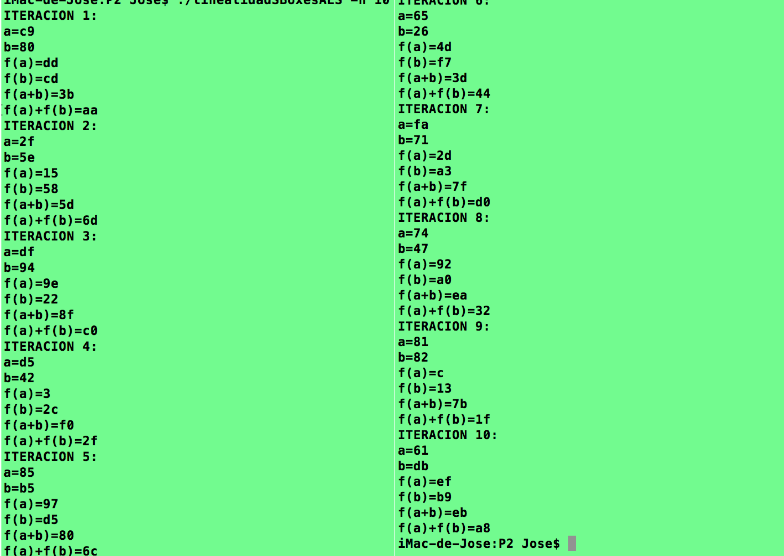
\includegraphics[width=400pt]{line1.png}
	\caption{No linealidad del AES}
\end{figure}

Para comprobar la nonlinealidad de las
SBOXES en ambos casos, basta con fijarse
en que se cumple la siguiente igualdad:
$$f(a)+f(b)=f(a+b)+K$$
Donde K sería lo que
llamaríamos constante
de no linealidad (si
fuese 0 la función sería
lineal).

En resumen, los principales criterios para construir unas buenas S-Boxes son los siguientes:
\begin{itemize}
	

\item \textbf{Balance}:Esta propiedad es muy deseable para evitar ataques cripto-diferenciales tales como los
introducidos por A. Shamir contra el algoritmo DES
\item \textbf{Alta no linealidad}: Esta propiedad reduce el efecto de los ataques por criptoanálisis lineal.
Como se discutió antes, la no linealidad de una función booleana puede ser calculada
directamente de la transformada de Walsh-Hadamard
\item \textbf{Autocorrelación}: Este valor es proporcional al desbalance de todas las derivadas de primer
orden de la función booleana. Valores pequeños son considerados como buenos mientras que un
valor grande es considerado un símbolo de debilidad.
Las funciones curvas gozan de una autocorrelación mínima, por lo que optimizan esta propiedad.• Indicador absoluto: Indicador absoluto de una función booleana denotado por M(f) está dado por
$|r_max|$ el máximo valor absoluto en $r_{\widehat{f}}(s)$ . Se considera que una función booleana con un M(f)
pequeño es criptográficamente deseable. Nuevamente las funciones curvas son las mejores, ya
que su indicador absoluto es 0.
\item \textbf{Efecto avalancha}: Está relacionado con la autocorrelación y se define con respecto a un bit
específico de entrada tal que al complementarlo resulta en un cambio en el bit de salida con una
probabilidad de 1/2. El criterio de avalancha estricto (SAC por sus siglas en inglés), requiere los
efectos avalancha de todos los bits de entrada. Se dice que una función booleana satisface el
criterio de avalancha estricto si al complementar un solo bit de entrada resulta en un cambio en un
bit de salida con una probabilidad de 1/2. Puede demostrarse fácilmente que una función booleana
f con función de autocorrelación $r_{\widehat{f}}(s)$  , satisface el criterio de avalancha estricto si y sólo si $r_{\widehat{f}}(s)$= 0 para toda s con peso de Hamming H(s)=1
\end{itemize}
\newpage
\section{Ejercicio 3a - SAC y BIC para las cajas-S del DES}

Primero vamos a explicar qué es cada uno de estos principios.

\begin{itemize}
	
	\item \textbf{SAC} (Strict avalanch criterion)
	
	Este principio dice que la probabilidad de cambio debe estar equidistribuida.
	
	Esto es, que si cambio un bit de entrada, la probabilidad de que un bit de salida sea 0 o 1 es la misma.
	$$\forall i,j\text{  }P(c_i=1|\overline{b_j})= P(c_i=0|\overline{b_j}) = \frac{1}{2}$$
	Siendo $\overline{b_j}$ que he cambiado el bit $b_j$
	
	\item \textbf{BIC} (bit independence criterion)
	
	Busca que no haya dependencia entre los bits de salida (si cambia $c_3$, no condiciona a que cambie o no $c_2$) 
	$$\forall i,j,k \text{  } P(c_ic_j|\overline{b_k}) = P(c_i|\overline{b_k})\cdot P(c_j|\overline{b_k})$$
\end{itemize} 	

Hemos hecho un programa que genera entradas aleatorias para lass cajas-S del DES.
Recorremos cada una de esas entradas, cambiando uno a uno sus bits y vemos cómo reacciona la salida ante estos cambios.

Los resultados que aparecen por pantalla para comprobar el criterio SAC están en el siguiente formato:

$$prob0[i][j] = ...$$
$$prob1[i][j] = ...$$

Que son la probabilidad de que el bit i sea 0 o 1 si cambio el bit j.

Los resultados que nos dan son cercanos a $0.5$ pero no son completamente satisfactorios.

\begin{center}
	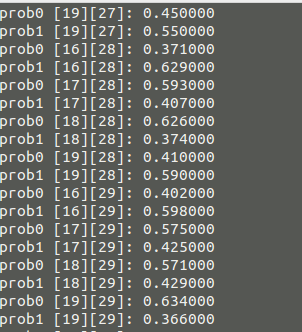
\includegraphics[width=200pt]{SACBIC_DESmod.png}
\end{center}

El criterio BIC lo hemos calculado no como pone en la definición sino:
$$P(c_ic_jc_kc_l|\overline{b_k}) = P(c_i|\overline{b_k})\cdot P(c_j|\overline{b_k})\cdot P(c_k|\overline{b_k})\cdot P(c_l|\overline{b_k})$$

El resultado lo escribimos en el formato $probsij[i][j] = ...$, donde $i$ va de 0 a 15 , que son los posibles valores que puedo escribir con $c_ic_jc_kc_l$ y j va de 0 a 47, que son los bits de la entrada.

\begin{center}
	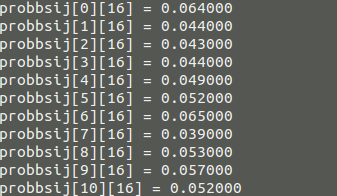
\includegraphics[width=200pt]{BICDES.png}
\end{center}

Vemos que este resultado tampoco es muy bueno ya que nos debería dar un número cercano a $0.0625 = 0.5^4$


\section{Ejercicio 4c - SAC y BIC para las cajas-S del AES}

El programa que hemos implementado para comprobar estos criterios es muy parecido al del DES.

En este caso hemos obtenido resultados mucho más satisfactorios.

Los resultados de SAC son los siguientes:
\begin{center}
	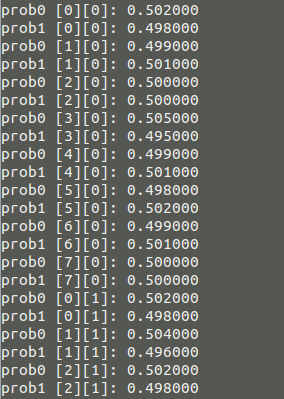
\includegraphics[width=200pt]{SACAES.png}
\end{center}

Sabemos que la S-caja del Rijndael  no satisface de manera directa el criterio de avalancha estricto,pero si dentro de una pequeña región de error.

Dicho error es $0.125$ y nuestros resultados están dentro de este error.

Los resultados del BIC son los siguientes:
\begin{center}
	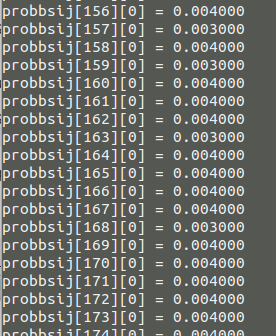
\includegraphics[width=200pt]{BICAES.png}
\end{center}

Vemos que $0.0039 = 0.5^8$ por lo que el AES cumple el principio de BIC.
\printindex
\end{document}